\documentclass[syuuron]{kuee}
\usepackage[dvipdfmx]{graphicx}
\usepackage{kueecite}

\title{評価構造における単語間の関係性可視化に関する研究}
\author{小澤 啓太}
\professor{小山田 耕二 教授}
\course{京都大学大学院 工学研究科}
\department{電気工学専攻}
\date{平成28年2月4日}

%%% 本文
\begin{document}
\maketitle
\tableofcontents


%%%序論
\chapter{序論}
	%%%人々の評価を解明するって大事!
	人々の価値観が多様化している現代社会において,人々が物事をどのように評価するか、
	何故そのように評価するかという評価の解明が意思決定に必要不可欠となってきた.
	現在、多くの企業にとって市場は自国だけでなく世界全体へと移行しつつあり、
	消費者の好みは年齢や性別、経済力だけでなく国、宗教などによって多様化している. 
	多様化により、商品のターゲット設定も具体的になる傾向にあり、より精度の高いマーケティング・リサーチが企業体には必要となっている. 
	精度の高いマーケティング・リサーチには、意思決定の結果がどのような効果をもたらすかをエビデンスを用いて議論するエビデンスベースな意思決定が必要である.
	エビデンスベースな意思決定技術の確立は,企業体での意思決定だけでなく国家や個人の意思決定の質の向上という意味でも重要性が高くなってきている.
	
	%%%人々の評価を解明する評価グリッド法とは?
	人々の評価を解明する手法の一つに評価グリッド法という, 半構造化インタビューを用いた定性調査手法がある. 
	評価グリッド法は、環境心理学やマーケティング調査、感性工学といった分野で日本を中心に幅広く利用されており、
	人間が何を知覚して, その知覚からどのような理解をし, どのような価値を見出しているのかという、ある対象物への評価構造を把握することができる.
	評価構造は「良い、悪い」等,価値判断に寄与している理解の単位 (評価項目) と,評価項目の間に存在する因果関係から構成され, 
	概観を可能にするためネットワーク図として表現されることがある(図~\ref{fig:es1}).
	ネットワーク図で表す場合, 図~\ref{fig:es2}のように頂点は評価項目を表しており,文章でラベル付けされている.
	また, 評価項目間の因果関係をネットワーク図の枝で表現する. 
	マーケティング分野などでは, この評価構造を分析することで,人間の価値観を把握でき, 人間の求める商品の推測につながるので、
	評価構造の効果的な分析方法に関する要求が高まっている\cite{egm6, egm7}.
	評価構造の分析に関する研究は数多く行われている~\cite{egm8, egm9}. 
	従来の評価構造は、模造紙や付箋などに手書きすることで作成される場合が多く、作成者の大きな負担となっていた. 
	しかし、近年ではE-grid\footnote{http://egrid.jp}のような, 評価グリッド法のインタビューと分析をサポートするWebアプリケーションも開発され, 評価構造作成の効率化が進んでいる~\cite{egm5, egm6}. 
	
	%%%従来での問題
	E-gridのような評価グリッド法を支援するアプリケーションが増加し評価構造作成の効率化が進む一方で、問題も発生している. 
	それは、評価構造の大規模化に伴う見やすさの低下、それによる評価構造分析の非効率化である. 
	従来の手書きでの作成では大人数の評価構造の統合などが困難であったが、Webアプリケーションなどの登場により容易に行えるようになった. 
	大人数の評価構造が統合されることで、評価項目数が増加し, 指定された領域内で評価構造全体を表示するには評価構造のレイアウトサイズを縮小する必要が発生した.  
	縮小された評価構造では、図~\ref{fig:es3}のように評価項目の文字や評価項目間の関係性が見づらくなる。
	評価構造を分析する際の着目点として, 評価構造内での頻出語の発見や頻出語と因果関係を持つ項目の把握があげられる. 
	評価構造内で頻出する単語とは、多くの人が回答した内容であり、多くの人が共有する価値観である. 
	また、頻出語と隣接する評価項目を知ることで、多くの人が共有する価値観の因果関係を知ることができる. 
	このように、頻出する評価項目や頻出語と隣接する評価項目を発見することで消費者の価値観を把握することができるが、
	縮小された評価構造では頻出語や評価項目間の関係性が見えづらく、分析を短時間で行うことが困難である. 	. 
	従来の評価構造分析手法では,評価構造を構成する評価項目間の因果関係に着目して因果関係の定量化を行う手法は数多く提案されている~\cite{egm8, egm9}. 
	しかし、評価構造の分析手法の多くはネットワーク図表示をもとにした分析である。
	ネットワーク図では上記のような見やすさに関する問題があるので、ネットワーク図以外での表示を行う必要がある。
	
	%%%提案手法!手法の説明, 実験の要約
	以上の問題を解決するために本論文は,評価項目内に出現する単語の頻度と,
	評価構造内での単語間の位置関係を反映した評価構造データ向けのテキストベースの可視化手法を提案し, 
	提案手法を用いた評価構造分析システムの開発を行った. 
	提案手法では,評価構造内の評価項目の文章を形態素解析し,抽出した単語をWord Cloud技術によって可視化する.
	Word Cloudとは文章中で出現頻度が高い単語を複数選び出し,その頻度に応じた大きさで図示する可視化技術である.
	また, 提案手法ではWord Cloud内の単語の配置座標を, 本論文で提案する評価構造内単語の座標計算手法を適用し決定した.
	提案する評価構造内単語の座標計算手法では, はじめに評価構造内での各単語間の位置関係をネットワーク図の最短距離を用いて計算する. 
	この単語の位置関係を多次元尺度構成法により二次元の値に縮小し, この値をWord Cloud内での単語の配置座標とする. 
	これにより、単語間の距離から因果関係を持つ項目の発見が容易になった。
	しかし, 単語の配置座標決定時は単語間の重複が発生し, 単語間の関係が分かりづらくなる可能性があるので, 
	単語間の位置関係を維持しつつ重複阻止を行った座標をWord Cloud内の単語の配置座標とした. 
	重複阻止では単語間の相対的位置関係の保持を行いつつ, 指定領域の最大活用するためのフォントサイズの最適化も行った. 
	これにより, 単語数に応じて最適なフォントサイズ, 評価構造内での単語の位置関係を保持した読みやすい可視化を達成した. 
	Word Cloudによる可視化は似た内容の評価項目の統合にもつながり,規模の大きい評価構造の場合でも分析を行いやすくなった.
	提案システムでは指定した単語の関係性を詳細に表示する機能や、評価構造のネットワーク図可視化とWord Cloud可視化を併置し、
	二つの可視化のインタラクティブな操作を可能にすることでより効率的な分析を可能とした. 

	%%%提案手法のもたらす効果
	本論文では, 評価構造のWord Cloud可視化の有効性, Word Cloud内の単語配置方法の有効性を検証するために二種類の比較実験を行った. 
	一つは, 評価構造のWord Cloud可視化の有効性を測るために比較実験である。 
	評価構造のネットワーク図とWord Cloud可視化による比較実験を行い、
	単語数が多い場合の評価構造の頻出単語の発見, 頻出語と因果関係を持つ単語の発見に関してWord Cloud可視化が有効であることを証明した. 
	もう一つは, Word Cloud内の単語配置方法の有効性を検証するため, 
	単語をランダムに配置した場合と提案手法に基づき配置位置を決定した場合とでの比較実験を行った. 
	比較実験により, 頻出単語の発見が容易になり, 単語の座標関係から頻出語と因果関係の強い単語の把握に有効であることが証明された. 
	また、提案システムの評価として提案システムを用い評価構造の分析を行ってもらい、その後にシステムに関するアンケートを行った. 
	提案システムによって多くの人の共有する評価基準や, その因果関係の分析に大きく貢献することが期待される. 

	%%%論文構成
	本論文の構成は以下の通りである.
	第1章は,本論文の序論である.第2章は,本論文の関連する研究について述べる. 第3章では,提案手法と使用するデータの説明を行う.
	第4章では、開発した提案システムについての詳細を述べる。
	第5章では,提案手法、提案システムを用いた評価実験の内容を述べる. 
	第6章では第5章で行った評価実験の結果を, 第7章では, 実験をもとにした考察を行う. 
	最後に, 第8章では本論文の結論と今後の課題について述べる.

		\begin{figure}
			\begin{center}
				\fbox{
				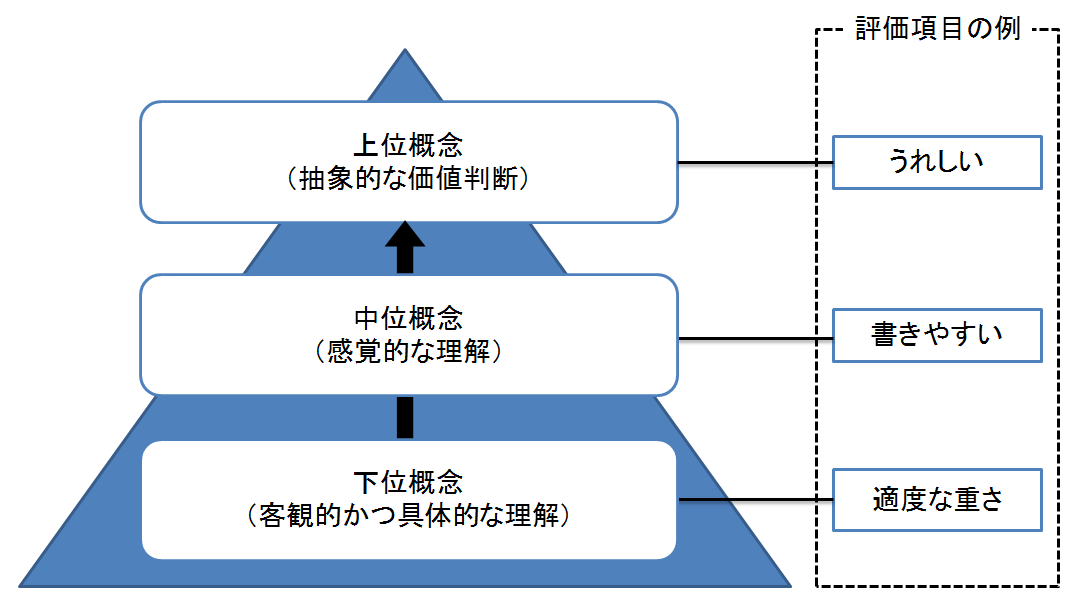
\includegraphics[width=\linewidth]{./png/es1.png}
				}
			\end{center}
			\caption{評価構造の構成}
	  		\label{fig:es1}
		\end{figure}
		\begin{figure}
			\begin{center}
				\fbox{
				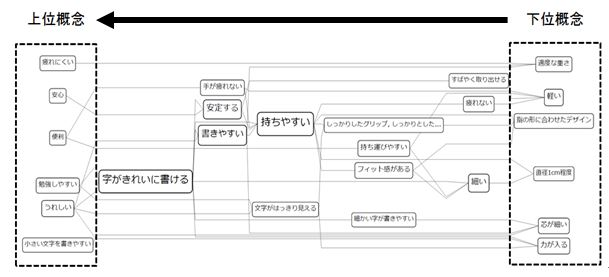
\includegraphics[width=\linewidth]{./png/es2.JPG}
				}
			\end{center}
			\caption{評価構造1}
	  		\label{fig:es2}
		\end{figure}
		\begin{figure}
			\begin{center}
				\fbox{
				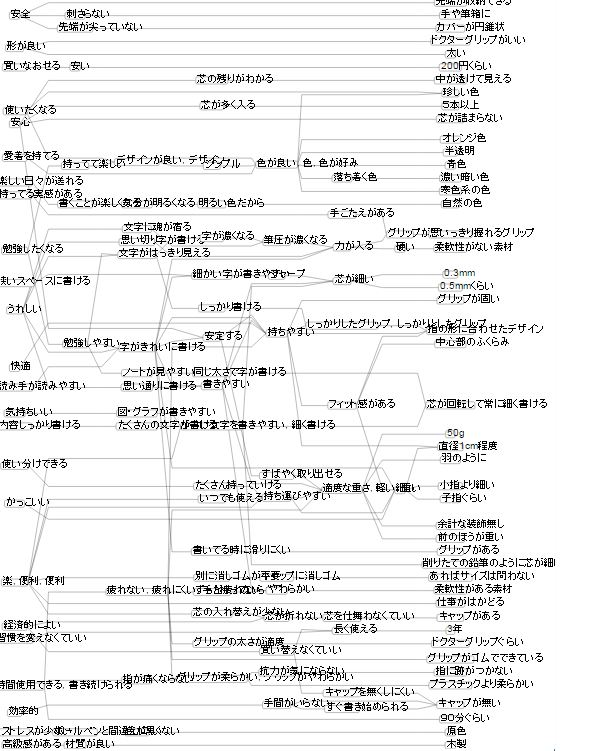
\includegraphics[width=\linewidth]{./png/es3.JPG}
				}
			\end{center}
			\caption{評価構造2}
	  		\label{fig:es3}
		\end{figure}

%%%関連研究
\chapter{関連研究}
	本研究では, 評価構造の文章の頻出語や関係性を可視化する. 本章では, 評価構造と評価構造を作成する評価グリッド法に関する研究, 
	テキストデータ内の頻出語や関係性の可視化に関する研究, 評価構造をWord Cloudで可視化する際に使用する単語の重複阻止法に関する研究に分けて関連研究を述べる. 
	\section{評価構造と評価グリッド法}
		%%%評価グリッド法のインタビュー手法内での立ち位置
		評価グリッド法とは半構造化インタビュー手法であり、この手法によって引き出された価値判断のネットワークが評価構造である\cite{egm6, egm7}. 
		半構造化インタビューとは,質問の流れがある程度決まっているインタビューで,質問の流れが完全に固定された構造化インタビューと、
		一般的な自由形式の非構造化インタビューとの中間にあたるインタビュー手法である.
		評価グリッド法は、デプスインタビューでもあり、基本的に回答者とインタビュアーによる1対1の面談式インタビューを行い、
		回答者が自覚していない深層心理を聞く事ができる. 
		
		%%%評価グリッド法の誕生話
		評価グリッド法は,レパートリー・グリッド法\cite{rg1}と呼ばれる臨床心理学の手法を元にしており,提案された当初はレパートリー・グリッド発展手法と呼ばれていた.
		レパートリー・グリッド法は各人が固有に持つ認知構造を抽出するために開発された面接調査手法である. 
		レパートリー・グリッド法は,被験者の認知構造の全体を抽出するためインタビューの時間が長く被験者の負担が大きいという問題が挙げられていた.
		そのため、評価グリッド法は認知構造のうち評価に関与する評価構造のみの抽出を行なうことで、問題とされていたインタビューを効率化した.
		また、評価構造には評価に関与する要素である評価項目が存在し、この評価項目の因果関係を明らかにするためにラダーリング法を取り入れることで,
		評価構造を階層ネットワーク構造として表現可能にした.
		
		%%%評価グリッド法の目的、適用先
		評価グリッド法は,人々が持つ認知構造のうち,ものごとへの評価に関する部分、
		すなわち人間がある対象をどのようなプロセスで理解し、評価していると考えるかを効率的に引き出すことを目的として開発された.
		評価グリッド法は,環境心理学分野で讃井らによって開発された手法であり、
		評価グリッド法の利用は環境心理学だけに留まらず,マーケティング調査や感性工学,魅力工学へと適用分野を広げてきた.
		マーケティング調査においては,評価グリッド法は商品企画七つ道具の一部として知られており,商品企画における顧客の潜在ニーズを調査するために実施される.
		感性工学及び魅力工学においては,評価グリッド法は製品の魅力を評価するための手法として位置づけられている. 
		
		%%%評価グリッド法の行い方
		評価グリッド法によるインタビュー手順はオリジナル評価項目の抽出とラダーリングの繰り返しである. 
		オリジナル評価項目とは, インタビューの起点となる評価項目であり, 
		ラダーリングとは, オリジナル評価項目からより抽象的な評価項目とより具体的な評価項目を引き出すための手順である. 
		インタビューにあたって, いくつかの調査対象を刺激要素として複数個準備しておく. 
		オリジナル評価項目の抽出では, 刺激要素の中から2つを回答者に提示し, どちらのほうが好ましいかを選択してもらう. 
		そして, 何故選択した要素のほうが好ましいと思ったのか理由を尋ね, 回答された理由をオリジナル評価項目として記録し, その回答をオリジナル評価項目としてグラフに描く.
		理由が複数個ある場合は, それらを全て記録する. 
		刺激要素が3個以上存在する場合は, インタビューの時間短縮のため, 回答者に刺激要素の好ましい順位をつけてもらい, 順位が隣り合う刺激要素を提示し, 
		オリジナル評価項目の抽出を行う場合がある. 
		ラダーリングでは, オリジナル評価項目からより抽象的な上位概念を引き出すラダーアップと, より具体的な下位概念を引き出すラダーダウンを行う. 
		ラダーアップでは, オリジナル評価項目としてあげられた理由「○○」について, 「〇〇だと何故いいのですか」と質問を行い, 回答された理由を上位概念として記録する. 
		さらに, 回答された上位概念についてラダーアップを行い, それ以上の上位概念が引き出せなく成るまで続ける. 
		ラダーダウンではラダーアップとは逆に, オリジナル評価項目としてあげられた理由「△△」について「具体的にどういうところが△△なのですか」と質問を行い, 
		回答された理由を下位概念として記録する. 
		そして, ラダーアップと同様に, 引き出された下位概念についてさらにラダーダウンを行い, それ以上の下位概念が引き出せなく成るまで繰り返す. 
		途中で理由が複数個挙げられた場合は, 上位概念または下位概念を枝分かれさせつつ上述の手順を繰り返す. 
		ラダリングで抽出したオリジナル評価項目の上位項目と下位項目はグラフにマッピングする.
		刺激要素全てのペアに対してオリジナル評価項目の抽出とラダーリングを行えばインタビューを終了する. 
		以上の手法を取ることにより,評価構造はある概念に対する評価を明らかにすることができるとされている. 
		
		%%%評価構造と評価グリッド法の関係
		評価グリッド法によって引き出された価値判断のネットワークを評価構造と呼ぶ.
		価値判断のネットワークとは,すなわち,人がある対象を評価する時に,どのような価値観を重視しているか,
		ある要素が満たされたときどのような価値観が満たされるか,ある価値観を満たすためにはどのような要素が必要であるかといった価値判断の接続関係である.
		評価グリッド法のインタビューは基本的には回答者と質問者の2人で行い,個人毎の評価構造図を作成する.
		その後,回答者全体の評価構造を把握する場合は,個人毎の評価構造を統合し全体の評価構造を作成する.
		また,評価構造中の価値判断の単位のことを評価項目と呼ぶ.
		評価グリッド法は,調査対象者の価値判断の全体像を把握する上で有効である.
		
		%%%評価構造に関する研究
		讃井らは人々の住環境に関する評価構造を作成し, 個人が持つ住環境評価の実態を明らかにした. 
		また, 評価グリッド法では個人毎の評価構造を統合し全体の評価構造を作成する場合もある. 
		その際, 評価構造内の評価項目間の因果関係について分析するために評価項目間の因果関係を定量化する分析手法が数多く提案された. 
		尾上らは, 満足度の高い学会についての因果関係を調べるため, 評価項目間の因果関係モデルの構築を行った\cite{egm8}. 
		評価グリッド法での結果からアンケート項目を設計及び実施し, アンケート結果をもとにグラフィカル連鎖モデリングを用いた因果関係モデルの構築と構造方程式モデリングによる分析を行った. 
		他にも, アンケート結果をもとに重回帰分析やパス解析, 階層分析, 共分散構造分析などを行う研究も提案されている. 
		本村らは, 評価グリッド法により抽出したスケルトン構造を基にしてベイジアンネットの統計的学習により定量的なモデルを構築し, 確率推論アルゴリズムの適用を行った\cite{egm9}. 
		
		%%%評価構造の新たな問題と自分の研究の立ち位置の説明
		評価グリッド法は, 従来は紙ベースで実施されることが多く, 分析作業などにおいて調査者の負担が大きかった. 
		しかし, 近年は評価グリッド法のインタビューと分析を支援するソフトウェアも開発され, 大人数の評価構造の統合が容易になった. 
		土田らが開発したEGM-assistは評価グリッド法支援ソフトウェアの代表例である。また、商品企画七つ道具の支援ソフトウェアである。PLANPARTERも評価グリッド法を支援している。
		以上のような評価グリッド法支援ソフトウェアは評価グリッド法に基づいたインタビューの効率化する。
		また、尾上はE-Gridという評価構造を分析するソフトウェアを提案している。
		以上のように評価構造の作成や統合が容易になることにより評価構造内のノード数が増え, 評価構造の概観や分析が困難になった. 
		評価構造を分析する場合ノードのラベルを読む必要があるが, 限られた領域に表示する必要があるので, 
		ノード数が増加するとノードの表示領域が小さくなり, ラベルの視認性が低下してしまう. 
		この問題に対して尾上らは評価項目数の削減を行った\cite{net1}. 
		各評価項目のネットワーク中心性を計算し, ネットワーク中心性の低い各評価項目を表示しないことで, 問題を解決した. 
		本論文は, 二つの方法から問題解決を行った. 
		一つ目の方法は助詞や助動詞などの意味無し語を排除. 二つ目の方法は評価構造内で複数回出現する単語の出現回数を一度に減少させることで, 
		重要度が低いが意味を持つ単語の領域を確保しつつ、従来より視認性の高い評価構造の可視化に成功した. 
		
	\section{テキストデータ分析}
		%%%テキストデータ分析の概要と例
		本研究では前節で述べたように, 評価構造が持つテキストデータを分析することで、
		頻出単語の発見, 頻出語と強い関係を持つ単語の発見することを目的としている.  
		テキストデータ分析は共起分析やテキスト要約など様々な目的のもと行われており、
		KH Coder\footnote{http://khc.sourceforge.net/}のような、テキストデータを統計的に分析するためのフリーソフトウェアも開発されている. 
		
		%%%テキストデータ分析の歴史
		KH Coderのようなコンピュータを用いたテキストデータ分析は古くから数多く提案されてきた. 
		1960年台の後半には、既に2つのテキスト分析アプローチが提案されていた. 
		一つはDictionary-basedアプローチと呼ばれ、分析者が分類基準を作成し、
		分析者の持つ理論や問題意識を操作化するためのアプローチである. 
		Dictionary-basedアプローチはコーディング規則を設けることで、データを絞り、様々な側面からデータを見ることができるという利点である. 
		その反面、意図的に理論や仮説に都合の良いコーディングが作成される危険も存在する. 
		もう一つは、Correlationalアプローチと呼ばれるもので、分析者の理論仮説や問題意識により汚染されていない状態で、
		多変量解析などによってコンピュータにデータ分析してもらうアプローチである. 
		近年では、この二つのアプローチを統合したアプローチが提案されている\cite{kh1}. 
		はじめにCorrelationalアプローチによりデータ全体を要約し、その結果を元にコーディングを作成する手順を踏むことで、
		分析者の持つ理論や問題意識の影響を極力受けない形でデータを分析することが可能となる. 
		提案手法も同様に二つのアプローチからテキスト分析を行う. 
		
		%%%テキストデータ分析の順序
		Dictionary-basedアプローチに関する研究は数多く行われている. 
		テキスト内で頻出する特徴語を抽出することや、語と語の関係性を調査するために階層クラスター分析や共起ネットワークを行う手法、
		内容が似た文書の群を探すクラスター分析など多岐にわたる. 
		提案手法では、前章で述べたように評価構造内の頻出語や単語間の関係性の分析を行うための可視化を行うことを目的としている。
		そこで提案手法では、はじめにDictionary-basedアプローチとして評価構造内の頻出語や単語間の関係性を可視化し、
		次にCorrelationalアプローチとして選択した単語の共起語の強調表示などを行った. 
		
		%%%出現頻度分析の例
		単語の出現回数の可視化に関して, Word Cloudのように単語の出現回数と単語のフォントサイズを比例させる手法が多く提案されている\cite{wc1}. 
		bubble chartでは単語の中心を中心点とし円を描き, 単語の出現回数と円の大きさを比例させている. 
		また, 出現回数順にリスト表示する手法なども活用されている. 
		
		%%%単語間の関係性分析の例
		テキストデータ内の単語の関係性の可視化に関して, ネットワーク可視化や多次元尺度構成法などが挙げられる. 
		ネットワーク可視化は, 共起した単語間に線を引く共起ネットワークなど, 数多く提案されている. 
		RiehmannらはWORDGRAPHというネットワーク図を用いたワイルドカードを含むkeyword-in-context検索結果を可視化する例文検索ツールを提案した\cite{wg1}. 
		WORDGRAPHでは検索結果に合致した文章を図~\ref{fig:es2}のように可視化する. 
		検索結果では例文に下線を引き, 各例文で共起する単語が存在する場合に, 共起単語の下線をまとめることで見やすさを向上した. 
		また、Wattenbergらもkeyword-in-context検索結果を可視化するWordTreeを提案した\cite{wt1}。
		WordTreeではでは利用者はツリー構造上に可視化される検索結果を対話的に操作することで利用者は文章を探索することができる。
		FrankらはPhrase netを提案し、構造化されていないテキストの可視化を行った\cite{pn1}。
		Phrase netでは、重複阻止する力指向レイアウトを用いて文書に出現する単語の組み合わせのパターンを可視化した。
		Carstenらはjigsawという複数のテキスト分析アルゴリズムを統合し対話的に可視化を行うことができる文書探索支援ソフトウェアを提案した\cite{jig1}。
		jigsawではテキスト可視化画面など複数の画面を表示することで文書の要約を容易にした。
		多次元尺度構成法では, 高次元属性を持つ分類対象物を低次元空間における点の布置で表現する手法であり, 点間の距離で関係性を表す. 
		Erickらは次元削減を用いたWeb検索結果の可視化を行った\cite{or1}. 
		検索結果のページのテキストデータからそれぞれ文書ベクトルを生成し, 次元削減を行うことで文書ベクトルが近い検索ページが近くに配置される. 
		同時に, クラスタリングを行うことで, 検索結果に複数分野の情報がある場合に目的の分野の情報を発見しやすくなった. 
		
		ネットワーク図では, 従来のようにノード数が増加する場合にエッジ数も同様に増加し, 全てを表示することで視認性が低下するので, 
		提案手法ではWord Cloudで可視化した. 
		Word Cloudによる可視化は意味無し語の削減だけでなく、似た内容の評価項目の統合にもつながり,
		規模の大きい評価構造の場合でも視認性が低下せず、分析を行いやすくなった.
		評価構造内での単語の関係性については、評価構造内での単語の距離関係から距離行列を作成し, 
		多次元尺度構成法を用いることで単語の座標を決定することで, 単語間の位置関係から評価構造内での単語の関係性を読み取れるようにした. 
		また, 提案手法を用いたシステムでは利用者が単語を選択すると選択単語が出現する評価項目の上位概念, 
		下位概念の単語との関係を可視化する機能を加えることで単語の関係性を読み取れるようにした.
		以上のように, Word Cloudを用いて必要最低限の情報のみを可視化することで, 単語の関係性の情報を残しつつ視認性が低下することを防いだ. 
		
	\section{重複阻止}
		%%%重複阻止の概要
		前節では、テキストベースの可視化の一つとして、単語の位置座標を計算したWord Cloudによる可視化について触れた. 
		提案手法のように、多次元データを次元削減し、低次元空間に配置する際、複数の対象が重複することは問題とされている. 
		このような重複問題は、ネットワーク表示でも問題とされており、重複阻止手法は古くから研究がされている. 
		重複阻止に関する研究では、以下の美的基準のいずれかを考慮したレイアウトを生成する. 
		\begin{itemize}
			\item 対象の相対的位置関係を保持する
			\item 対象間の距離関係を維持する
			\item 指定された領域からはみ出さない
			\item 指定領域の空白部分を減らす
		\end{itemize}
		
		%%%重複阻止その1(fta論文参考)
		重複阻止手法では大きく三種類のアプローチが提案されていた. 
		一つ目は、均等スケーリングである. 均等スケーリングでは、図形やオブジェクトを全ての方向に同じ倍率で拡大または縮小するアプローチである\cite{fsa1}. 
		このアプローチでは、オブジェクトの相対的位置関係や距離関係は維持されるものの、図形やオブジェクトを不必要に移動させる必要があり、
		指定領域を大幅に拡大する必要が出てくるという問題が発生する. 
		
		%%%重複阻止その2
		二つ目のアプローチは、力学モデルである. 
		力学モデルでは、グラフを対象としており、グラフの頂点と辺に仮想的な力を割り当て、力学的エネルギーの低い安定状態を探すことで重複を阻止する. 
		XiaodiらはForce Transfer algorithm(FTA)を提案した\cite{fta1}.
		FTAでは一定の規則に基づきオブジェクトを選択し, 重複オブジェクトが存在するか調べる. 
		重複オブジェクトを発見した場合, 重複オブジェクトを水平方向か垂直方向かに移動させる力を発生させる. 
		移動する方向は重複が解除されるまでに移動する距離が短い方向を選択する. 移動したオブジェクトと重複する他のオブジェクトも同距離同方向に移動する. 
		移動が終わったら他のオブジェクトを探し, 同様の操作を行う. 以上の操作を繰り返す手法である. 
		FTAでは、対象間の距離関係を維持した重複阻止が達成された. 
		StrobeltらはRWordle-Cを提案した\cite{rwc1}. 
		RWordle-CはFTAと同様に一定の規則に基づきノードを選択し, 重複ノードの有無を調べ, 
		重複ノードを発見した場合, 重複ノードを渦状に移動させる. 初期位置を渦の中心とし広がるように移動させ, 重複が解除される位置まで移動させる. 
		力学モデルを用いた重複阻止では、均等スケーリングに比べ、レイアウトがコンパクトになる利点があるが、
		上記の力学モデルをWord Cloudに適用すると, 単語の文字列の方向と重複阻止のために移動する方向の相関が強く, 
		指定領域をはみ出すことや, 指定領域内に空白部分が多く残るという問題が発生する. 
		そこで, 提案手法では三つ目の条件付き最適化を適用した. 
		
		%%%重複阻止その3
		条件付き最適化では、重複問題を制約条件を用いた最適化計算に置き換えることで重複を阻止する. 
		Erickらは, 可視化対象の座標を変数とした目的関数を作成し座標を計算する手法を提案した\cite{or1}. 
		NEIGHBORHOOD PRESERVING SNIPPET LAYOUTでは, 目的関数に重複阻止と単語の距離関係の維持を目的とした関数を作成することで
		対象間の距離関係を保持しつつ. 重複の発生しない座標計算を可能とした. 
		また, Erickらは目的関数に, 制約条件を追加した最適化手法も提案している\cite{or2}.  
		可視化対象は二次元空間に配置されている点群であり、はじめに指定領域内で格子を生成し, 格子内で座標点が存在する四角(細胞)だけを残し, 
		細胞のx,y座標、細胞の辺長を変数として最適化する. 
		最適化計算を行う際に, 相対的位置関係保持, 細胞間の重複阻止, 指定領域の最大利用, 指定領域外への細胞のはみ出し禁止など, 
		複数の制約条件を設けることで適切な細胞配置を可能にした. 
		このように、条件付き最適化では複数の美的基準を制約条件に置き換えることで様々な条件を満たした重複阻止を可能とする. 
		提案手法ではErickらが提案したエネルギー関数を用いた重複阻止の最適化計算手法を参考にし、
		Word Cloudで表示する単語内の1文字を格子の1細胞と置き換え, 細胞の位置の最適化計算を行った. 
		また, Erickらの制約条件を一部修正し新制約条件を追加することでWord Cloudでの単語配置に適した座標計算を可能とした. 

%%%本提案システム
\chapter{提案手法}
	本章では, 提案手法である、評価構造のテキストデータから単語のWord Cloud内座標を計算するまでのプロセスと使用する評価構造のテキストデータの説明を行う. 
	
	\section{使用データ}
		評価構造データ向けのテキストベース可視化を行うにあたって,評価グリッド法による評価構造データの作成を行った.
		本研究では, E-Gridを用いて評価構造データの作成を行った. 
		E-Gridとは, 評価グリッド法に基づいた評価構造の抽出や分析をビジュアル的に支援するシステムであり, 
		評価構造を抽出する機能から評価構造データを作成した. 
		E-Gridでのインタビューは1人ずつで行い,個人の評価構造を作成した.
		その後,回答者全体の評価構造を把握するため,個人毎の評価構造を統合し全体の評価構造を作成した.
		E-Gridにより作成される評価構造データは評価項目と隣接する評価項目,評価項目の回答者数 (=重み) ,評価項目のテキストラベル, 評価項目の回答者名等の情報を記載されている.
		提案する可視化手法は評価項目の重み,隣接する評価項目の情報,評価項目内のテキストラベルの情報を使用する.
		提案手法では文章ではなく単語ごとに可視化する必要があるので,テキストラベルに形態素解析を行った. 
		形態素解析には日本語形態素解析システムMeCab\cite{mcb1}と形態素解析辞書Unidicを使用した.
		Unidicは, 語彙素・語形・書字形・発音形の階層構造を持つので,表記の揺れや語形の変異にかかわらず同一の単語と識別することが可能である. 
		提案手法では, 表記の揺れや語形の変異がある単語はそれぞれの単語の語彙素を表示する. 
		形態素解析により抽出した単語の中で品詞が名詞・動詞・形容詞のいずれかである単語を提案システムでは使用する. 
		以上から得られたデータに以下のプロセスを通し可視化を行う. 
		
	\section{座標計算}
		提案システムでの可視化プロセスは大きく3つに分けられる. 
		はじめに, 評価構造データから評価構造内単語間の距離行列を作成する. 
		次に, 評価構造内単語間の距離関係を保持したまま単語をWord Cloud可視化するため, 次元削減法を用いて各単語のx, y座標を計算する. 
		計算した座標では単語間の重複が発生する場合があるので, 
		単語の重複を排除し, しかし単語間の位置関係を崩さず, 指定領域を最大限活かすことのできる単語の座標を再計算する. 
		Word Cloudに可視化する際は再計算された座標を使用する. 
		以下の項では, 可視化プロセスの詳細を説明する. 
		
		\subsection{単語間距離行列の作成}
			前章で記述したとおり,提案手法ではWord Cloud内の単語の座標を評価構造内での単語の距離関係を考慮して決定する.
			評価構造内単語間の距離関係は単語が使用されているノードの距離関係から計算され,単語間距離行列Dで表す.
			単語間距離行列Dは,評価構造から計算される出現行列F,ノード間距離行列U,重み行列A から計算される.
			Fig?は評価構造と評価構造から取得された出現行列F,ノード間距離行列U,重み行列Aの例を表す.
			以下ではノード間距離行列U,出現行列F,重み行列Aの導出方法を述べる.
			$ノード群はN \in {n_{1}, n_{2}, ..., n_{l}}, 単語群はW \in {w_{1}, w_{2}, ..., w_{m}}, で表す。$
			$またノードn_iを回答した人数をa_i、単語w_iの全ノードでの使用回数をu_iと表す。$
			
			\subsubsection{ノード間距離行列}
				ノード間距離行列Uは,各ノード間の距離関係を表す行列である. 
				ネットワーク図のノードViとVjの最短距離の経路でノードをn個経由する場合, 
				第i行第j列と第j行第i列の要素がn+1となる行列である.
				また、対角成分の値は全て0である。
				最短経路の計算は幅優先探索アルゴリズムを使用した. 
				このアルゴリズムは横型探索とも言われ, 以下のルールに従って探索を行う. 
				
				\begin{enumerate}
					\item 根ノードを空のキューに加える. 
					\item ノードをキューの先頭から取り出し, 以下の処理を行う. 
						\begin{itemize}
							\item ノードが探索対象であれば, 探索をやめ結果を返す. 
							\item そうでない場合, ノードの子で未探索のものを全てキューに追加する. 
						\end{itemize}
					\item もしキューが空ならば, グラフ内の全てのノードに対して処理が行われたので, 探索をやめ"not found"と結果を返す. 
					\item 2に戻る. 
				\end{enumerate}
				
				\begin{eqnarray}
				 U = \left(
				    \begin{array}{cccc}
				    	u_{11} & \ldots & u_{1l} \\
				    	\vdots & \ddots & \vdots \\
				    	u_{l1} & \ldots & u_{ll}
					\end{array}
				 \right)
				\end{eqnarray}	
		
			\subsubsection{出現行列}
				出現行列Fはノードと単語の関係を表す行列である.
				出現行列の列は評価構造内のノードを, 行は全ノードから形態素解析を行い取り出したの全ての単語群を表す. 
				i行目の単語がj列目のノードの文章に出現しない場合は0となる.
				出現する場合、i行目の単語がn個のノードで使用されていると第i行第j列の要素は1/nとなる。
				要素の値を使用回数の逆数とすることで単語が複数のノードで出現する際に単語間距離を平均の距離となる。
				この行列から各ノードに出現する単語を知ることができる. 
				\begin{eqnarray}
				 F = \left(
				    \begin{array}{cccc}
				    	f_{11} & \ldots & f_{1l} \\
				    	\vdots & \ddots & \vdots \\
				    	f_{m1} & \ldots & f_{ml}
					\end{array}
				 \right)
				\end{eqnarray}	
				\[
				  f_{ij} = \left\{ \begin{array}{ll}
				    \frac{1}{u_i} & (n_i \in w_j) \\
				    0 & (otherwise)
				  \end{array} \right.
				\]
				
			\subsubsection{重み行列}
				各ノードの重み行列Aは,各ノードの回答者数を表す行列である.
				対角成分以外の値は全て0とし、対角成分は回答者数の逆数とする。
				i番目のノードの回答者数がnの場合、第i行第i列の要素は1/nとなる。
				提案手法では、頻出語の関係性をより詳細に可視化するため、頻出語ほど距離行列の値が小さくなるよう設定した。
				\begin{eqnarray}
				 A = \left(
				    \begin{array}{cccc}
				    	a_{11} & \ldots & a_{1l} \\
				    	\vdots & \ddots & \vdots \\
				    	a_{l1} & \ldots & a_{ll}
					\end{array}
				 \right)
				\end{eqnarray}
				\[
				  a_{ij} = \left\{ \begin{array}{ll}
				     0 & (i ≠ j) \\
				     \frac{1}{a_i} & (i = j)
				  \end{array} \right.
				\]
				
				
			上記の3行列F,U,Aを計算した後,以下の式によって単語間距離行列Dを計算する.
			$ネットワーク図内の単語w_iとw_jの最短距離の平均値が, $
			第i行第j列と第j行第i列の値となる行列である.
			\begin{eqnarray}
			 D = \frac{1}{2} FAUA^{\mathrm{T}}F^{\mathrm{T}}
			   = \left(
			    \begin{array}{cccc}
			    	d_{11} & \ldots & d_{1m} \\
			    	\vdots & \ddots & \vdots \\
			    	d_{m1} & \ldots & d_{mm}
				\end{array}
			 \right)
			\end{eqnarray}	
			
		\subsection{次元削減}
			次に, 評価構造内単語間の距離関係を保持したまま単語をWord Cloud可視化するため, 単語のx, y軸の値を求めるために次元削減を行う.
			次元削減を行うことで,単語数の行と2列の行列式を計算し,この2次元の値を単語のx, y軸の値にする.
			提案システムでは多次元尺度構成法を適用することで次元削減を行う. 
			多次元尺度構成法とは, 多変量解析の一手法である.  分類対象物の関係を低次元空間における点の布置で表現する. 
			多次元尺度法では, 始めにヤング・ハウスホルダー変換を施す. 
			ヤング・ハウスホルダー変換は距離の2乗の行列に両側から中心化行列をかける演算であり, 以下の式で表す. 
			\begin{eqnarray}
				P = - \frac{1}{2} JDJ^{\mathrm{T}}
			\end{eqnarray}
			$単語数をnとすると, 行列Jは単位行列から全要素に1/nの行列を引いたn \times n行列を引いたn \times n行列$
			$行列Dは点 x_i と x_j の間の距離 d_{ij} の2乗を要素とするn×n行列である.$
			次に, Pをスペクトル分解することで固有値, 固有ベクトルを求め, 固有値の大きい方から2つ取り, 対応する固有ベクトルを取り出す. 
			各単語のx,y座標は取り出した2つの固有ベクトルの値となる. 
			
		\subsection{重複阻止}
			最後に, 計算した座標では単語間の重複が発生するので, 単語間の相対的位置関係を崩さないように単語の重なりの除去を行う. 
			提案手法ではErickらが提案した重複阻止手法を参考にした\cite{or2}. 
			Erickらの提案手法では指定領域内で格子を生成し, 格子の1区画を細胞と呼ぶ. 
			そして座標点が存在する細胞だけを残し, 細胞の位置座標を最適化計算する手法である. 
			この手法では, 細胞間の相対的位置関係保持, 細胞間の重複阻止, 指定領域の最大利用を達成する
			最適な細胞の座標を計算する. 
			提案手法では単語内の1文字を格子の1細胞, 各単語を細胞が隣接する長方形と置き換え, 単語の位置の最適化計算を行う. 
			提案手法では, 正方形の細胞ではなく長方形の細胞の座標最適化計算なので一部制約条件を修正した. 
			以下の節では最適化計算で用いる目的関数, 制約条件の説明を行う. 
			
			指定領域に配置する単語の集合を$G={g_1,g_2,…,g_n}$とし, 単語の各文字, 
			すなわち各細胞の集合を$H={h_{11},h_{12},…,h_{1m},h_{21},…,h_{nm}}$とする. 
			各細胞は正方形であり, $h_{ij}=(x_{ij},y_{ij},w_{ij})$で表される. 
			$(x_{ij},y_{ij})$は正方形 $g_{ij}$  の中心点, $w_{ij}>0$ は正方形 $g_{ij}$ の辺の長さである. 
			$w_{ij}$  は $w_{ij} = \alpha_i \delta $,$ \alpha_i $は $ \alpha_i=  e_i⁄(max⁡(e_1,e_2,…,e_n))$ と表し, 
			$e_i $ は単語 $ g_i $ の評価構造内での出現頻度を表す. 
			すなわち $w_{i1}= w_{i2}=⋯=w_{im}$ となる.$ \delta $ は再編成後の最頻出語の辺の長さを表す. 
			各細胞は縦, 横の辺の長さが $W × H$である指定領域内で細胞間の大きさの比率を維持しつつ, 
			細胞間の重複阻止と指定領域の最大利用, 細胞間の相対的位置関係の保持を達成するように再編成される. 
			
			\subsubsection{目的関数}
				指定領域内で単語を再編成するために, 提案手法では単語の再編成を以下のように最適化問題として定式化した.
				\begin{eqnarray}
					minimize\:\:   \sl{E(\bf{z})} = \sl{E_{comp}(\bf{z})} + \sl{E_{resize}(\bf{z})} \nonumber \\
					subject\: to\:\:   A \bf{z} \le \bf{b},   \bf{z} = [\bf{x} \: \bf{y} \: \bf{r} \: \bf{\delta}]^T, \nonumber \\
					\bf{x} = (x_1,x_2,...,x_N)^T \in \bf{R}^N \nonumber \\
					\bf{y} = (y_1,y_2,...,y_N)^T \in \bf{R}^N \\
					\bf{r} = (r_{12},...,r_{1N},r_{23},...,r_{2N},...,r_{N−1N})^T, 
					\bf{r_{ij}} \in {0,1} \nonumber \\
					\delta \le min(W,H) \nonumber,
				\end{eqnarray}				
				$\bf{z} は求める変数である$. 
				$ \bf{x}, \bf{y} は細胞の重心座標$,  $ \bf{r} は単語の重複を防ぐための調整変数, \delta は再編成後の最頻出語の辺の長さを表す変数である$. 
				$A, \bf{b} は最適化問題の制約条件を表す行列である$. 
				$エネルギー項 \sl{E_{comp}(\bf{z})},  \sl{E_{resize}(\bf{z})} はそれぞれ単語と指定領域を操作する関数である$. 
				前者は単語間重複と相対的位置関係の保持を考慮する単語集約エネルギー項, 後者は指定領域を可能な限り最大利用するための指定領域最大利用エネルギー項である. 
				以下では2つのエネルギー項についての詳細を述べる. 
			
				\paragraph{単語集約エネルギー項}
					一つ目のエネルギー関数 $\sl{E_{comp}(\bf{z})} $ は単語集約エネルギー項であり, 
					この関数の目的は細胞を狭い範囲で簡潔に表すことである. 
					エネルギー関数$ \sl{E_{comp}(\bf{z})} $は, 細胞の重心座標を変数とした二次間数で以下の式で表す. 
					\begin{eqnarray}
						\sl{E_{comp}(\bf{z})} = C \sum_{(i,j)} {{(x_i - x_j)^2 + (y_i - y_j)^2} },\\
						C = \frac{1} {( min(W,H) \times \frac{n(n-1)} {2} )},\nonumber
					\end{eqnarray}			
					$(i,j)=(j,i) は単語 (g_i, g_j), i, j \in {1,2,…,n}の組み合わせを表す.$ 
					$x_i, y_i は単語g_iの重心点の座標であり, x_i = \frac{\sum_{j} x_{ij}} {m}, y_i=  \frac{\sum_{j} y_{ij}} {m}で表す. $
					$n は単語数を表し,mは単語g_i  の文字数である. $
					Cは標準化のための定数であり, 指定領域最大利用エネルギー項との値の調節を行う. 
					$ \sl{E_{comp}(\bf{z})}は単語間の距離が短くなるほど小さくなり, 最小となるのは全単語の重心点が重なる場合である. $
				
				\paragraph{指定領域最大利用エネルギー項}
					$二つ目のエネルギー関数 \sl{E_{resize}(\bf{z})} は指定領域最大利用エネルギー項であり, 
					この関数の目的は指定領域を細胞で最大限満たすことである. $
					上記したように全ての細胞の辺の長さは, 最大の細胞の辺の長さに依存している. 
					そこで提案手法では指定領域最大利用エネルギー関数を以下の二次間数で表す. 
					\begin{eqnarray}
						\sl{E_{resize}(\bf{z})} = (\delta - min(W,H) )^2,
					\end{eqnarray}
					$min(W,H)とは指定領域の短辺の長さを表す. $
					$ \sl{E_{resize}(\bf{z})} は細胞の辺が長くなるほど小さくなり, 指定領域の短辺の長さと最大の細胞の辺の長さが等しい場合に 最小になる. $
					
				制約条件がない場合だと式(?)のエネルギー関数は全細胞の重心が重なり, 最大の細胞の辺の長さが指定領域短辺の長さと等しい場合が最小となる.
				この状況では単語重複が達成されていないので3つの制約条件を設けた. 
				次項では3つの制約条件の詳細を説明する. 
			
			\subsubsection{制約条件}
				$式(?)で表したように, A, \bf{b} は制約条件を表す行列であり, 重複阻止, 相対的位置関係, 指定領域からのはみ出しの阻止の保持を行う.$ 
				各単語の初期座標は$(x_i,y_i)$と与えられており, 
				単語の相対的位置関係を保存するための制約条件は以下で表される. 
				\begin{eqnarray}
					x_{p1} \le x_{p2} \le ... \le x_{pn} \Rightarrow x_{pi} - x_{pi+1} \le 0 \nonumber \\ 
					y_{p1} \le y_{p2} \le ... \le y_{pn} \Rightarrow y_{pi} - y_{pi+1} \le 0
				\end{eqnarray}
				$p, q : \bigl\{ 1,2,…,n \bigl\} \rightarrow \bigl\{ 1,2,…,n \bigl\} は単語の初期座標x_i,y_i を大きさ順に並び替えるために使用した. $
			
				重複阻止は以下の制約条件を用いて行われる. 				
				\begin{eqnarray}
					|x_j - x_i| \ge \frac{( \alpha_i n_i + \alpha_j n_j)} {2} \delta,\nonumber \\
					  or  \\
					|y_j - y_i| \ge \frac{( \alpha_i + \alpha_j)} {2} \delta,\nonumber 
				\end{eqnarray}
				$式(?)から x_j \ge x_i, y_j \ge y_i が成り立つ場合,|x_j - x_i|= x_j-x_i, |y_j - y_i| = y_j-y_iとなり, $
				式(?)は以下のように表すことができる.				
				\begin{eqnarray}
					x_j - x_i \le - \frac{( \alpha_i n_i + \alpha_j n_j)} {2} \delta,\nonumber \\
					 \: or \: \\
					y_j - y_i \le - \frac{( \alpha_i + \alpha_j)} {2} \delta,\nonumber 
				\end{eqnarray}
				$この数式の or 条件はバイナリ値r_{ij} \in \bigl\{0, 1 \bigl\}を用いて次式のように表すことができる. $
				\begin{eqnarray}
					x_j - x_i \le \alpha_{ij} \delta + M r_{ij} 
					\Leftrightarrow
					y_j - y_i \le \alpha_{ij} \delta + M(1 - r_{ij}) ,\\
					\alpha_{ij} = - \frac{(\alpha_i n_i + \alpha_j n_j)} {2}
				\end{eqnarray}
				$Mは値のとても大きい定数, n_iは単語iの文字数を表す.$
				$r_{ij}は式(?)の不等式の片方が成立する場合, もう片方の式を成立させる. $
				$例えば,  x_j - x_i \le \alpha_{ij} \delta が成り立つ場合, r_{ij}を0とする. $
				$その場合, y_j - y_i \le \alpha_{ij} \delta + M(1 - r_{ij})はyがどんな値であろうと成り立つ$
				
				最後に 単語が指定領域外に出ることを防ぐために以下の制約条件を設定した.
				\begin{eqnarray}
					0 \le x_i  -  \frac{a_i n_i} {2} \delta \:  and \:  x_i  +  \frac{a_i n_i} {2} \delta \le W, \nonumber \\
					0 \le y_i  -  \frac{a_i} {2} \delta  \: and \:  y_i  +  \frac{a_i} {2} \delta \le H ,\\
					i = 1, 2, ...,N, \nonumber
				\end{eqnarray}
				この3つの制約条件により, 重複阻止と指定領域の最大利用, 細胞間の相対的位置関係の保持を満たした単語の再編成が達成される. 
	
	\section{計算方法}
		提案手法では, 単語間距離行列を計算したが, この計算はpythonを用いた. 
		単語間距離行列を求めるためにノード間距離行列を求めたが, その際の幅優先探索はMATLABを用いて行った. 
				
		また, 提案手法では単語の重複阻止のために最適化計算を行っており, この計算は混合整数二次計画問題である. 
		最適化計算には, Gurobi Optimization Package\footnote{http://www.gurobi.com/}により提供されるソルバーGurobi Optimizerを用いて行った.
		Gurobi Optimizerでは, 最適化計算は混合整数二次計画問題は分枝限定法を使って解く. 
		分枝限定法とは最適化問題の最適解を求めるための汎用アルゴリズムであり, アルゴリズムは以下となる.
		$P_0$を最適化問題(最小値を求める問題), zを最適解の最小値, f(P)を目的関数の値, g(P)を目的関数の緩和問題の値とする. 
				
				\begin{enumerate}
					\item 初期設定: $A = {P_0}, z = ∞$
					\item $A = φ$ ならば終了.
						\begin{itemize}
						\item $z = ∞: 問題 P_0 は解を持たない$
						\item $z < ∞: f(P_0) = z$
						\end{itemize}
					\item $集合 A の中から,部分問題 P_i を選択$
					\item $もし,緩和問題 P'_i が解を持たなければ,$
					\begin{description}
						\item $A = A - {P_i} として,2 へ戻る$
					\end{description}
					そうでなけでば,
					\begin{description}
						\item $もし,g(P'_i) = f(P_i) として,P_i の最適値が得られたら,$
						\begin{description}
							\item $z = min \bigl\{z, f(P_i)\bigr\}, A = A - {P_i} として,2 へ戻る.$
						\end{description}
						\item そうでなければ
						\begin{description}
							\item $もし,g(P'_i) ≧ z ならば$
							\begin{description}
								\item $A = A - {P_i} として,2へ戻る.$
							\end{description}
							\item そうでなければ
							\begin{description}
								\item $問題P_iを,部分問題 P_{i1}, ..., P_{ik} に分解し, A = (A - {P_i}) ∪ \bigl\{ P_{i1}, ..., P_{ik} \bigr\} として,2へ戻る.$
							\end{description}
						\end{description}
					\end{description}
				\end{enumerate}
% https://www.sist.ac.jp/~suganuma/kougi/other_lecture/SE/opt/combination/combination.htm
% http://ideas.paunix.org/latex/latex_6_list.htm

%%提案システム
\chapter{提案システム}
	\section{システム要件}
		本節では, 評価グリッド法の専門家のインタビュー結果\cite{hak1}を通して, 評価構造分析システムの要件を分析した. 
		以下では、インタビュー結果から得られた、評価構造分析に求められている機能を示す。
		\subsubsection{評価構造の全体を把握する}
			分析者はどのような単語や評価項目が評価構造内に現れているかに関心がある。
			頻出する単語、評価項目だけでなく一度しか出現しない単語、評価項目にも予想外の発見が存在する可能性はある。
			全体評価構造図を作成した後に、分析者は評価構造図を俯瞰し評価構造の全体像をつかむ。
			しかし、評価構造の規模が増大するに連れて評価構造の探索にかかる時間は増加し、
			見逃してしまう評価項目、情報が発生する可能性もある。
			評価構造図をコンパクトに表示し、対話的な操作を可能にすることは、
			評価構造の全体把握を行う上では重要である。
		\subsubsection{評価項目間の関係性を把握する}
			評価項目の上位概念、下位概念を知ることは個人が持つ価値観の因果関係を知ることである。
			この因果関係は評価構造が持つ重要な情報の一つである。
			評価項目間の関係性を知るためには、分析者は注目した評価項目と隣接する評価項目を探索する。
			評価構造の規模が大きくなるにつれ、評価項目間の関係は複雑になり、評価項目間の関係性は把握しづらくなる。
			そのため評価構造図の読みやすさは重要な要素であり、その関係を確認するためのインタラクションが必要となる。
		\subsubsection{重要な項目を特定する}
			評価構造は複数人の実験参加者が回答した評価項目が存在する。
			この評価項目は、多くの人が共有している評価基準であり、
			分析者にとってこの評価項目を特定することは重要な事である。
			重要な評価項目を見つけるためには、重要な評価項目を自動的に絞り込むことや強調表示することが必要となる。
		\subsubsection{実験参加者をグループ分けする}%%%尾上さんにグループ分けが必要な理由を聞きそれを記述
			実験参加者は異なる意見を持つグループに分けることができる場合があり、
			分析者は実験参加者をグループ分けできるかを試す。
			従来は、評価構造を手書きで作成しており、実験参加者が10人を超えるような
			規模の大きい評価構造の場合、グループ分けを行うのはかなりの時間を要した。
			そのため、実験参加者のグループ化を考慮した上で自動評価構造のレイアウトをすることが必要である。
		\subsubsection{評価項目をグループ分けする}%%%尾上さんにグループ分けが必要な理由を聞きそれを記述
			評価構造内の評価項目をグループ分けすることは分析において必要である。
			従来は、分析者が主観的に評価項目を分類し、グループを作成していたが、
			分析者の主観が入る場合があり、分析者によってグループ分けの結果が異なる場合がある。
			そのため、客観的な基準をもとにグループ分けを行う機能は必要である。
	\section{システム設計と実装}
		前節で述べたシステム要件をもとに、評価構造分析システムの開発を行った。
		本節では提案システムの設計と実装の詳細について述べる。
		\subsection{概要}
			図?は提案システムのスクリーンショットである。
			提案システムは3つの要素から構成されており、それぞれ評価構造ウィンドウ、Word Cloudウィンドウ、評価項目リストウィンドウである。
			評価構造ウィンドウでは、評価構造図を表示する。
			このウィンドウの目的は、評価構造内の評価項目間の関係性を直接見ることである。
			評価構造ウィンドウはWord Cloudウィンドウ、評価項目リストウィンドウと連動していて、
			あるウィンドウでの操作が即座に他のウィンドウに反映される。
			Word Cloudウィンドウでは提案手法を用いた評価構造内の評価項目で使用されている単語を表示する。
			Word Cloudウィンドウでの目的は、重要な単語の発見や、単語間の概括的な関係性の発見、評価構造の概要把握が挙げられる。
			評価項目リストウィンドウではWord Cloudウィンドウで選択した単語が使用されている評価項目を表示する。
			評価項目リストウィンドウの目的は、利用者が単語に注目した場合の詳細な情報を示すことである。
			提案システムの評価構造ウィンドウと評価項目リストウィンドウはE-Gridから得た評価構造データを用いて表示し、
			Word CloudウィンドウはE-Gridから得た評価構造データと提案手法を用いて作成したデータを用いて表示した。
			
			提案システムはHTMLやJavascriptといったWeb標準技術を用いて開発されたWebアプリケーションである。
			また、レイアウトの一部をbootstrapを用いて実装されており、タブレット端末のような画面の小さい装置や
			PCディスプレイ、タイルドディスプレイのような大画面好解像度での柔軟なレイアウトを可能にしている。
			
			システム要件と提案システムの機能は以下のように対応している。
			\subsubsection{評価構造の全体を把握する}
				利用者はWord Cloudウィンドウを見ることで評価構造の概要を把握することができる。
				頻出単語は大きく表示され、そうでない単語も助詞や助動詞などの意味なし語を表示しないため、
				ネットワーク図で全体を表示した場合よりもフォントサイズが大きい場合が多い。				
			\subsubsection{評価項目間の関係性を把握する}
				利用者はWord Cloudウィンドウ内の単語の位置関係から評価項目内の単語間の関係を把握することができる。
				また、その中から注目したい単語を選択することで、注目した単語と共起する単語、
				評価構造内で隣接関係にある評価項目の単語を知ることができる。
				また、Word Cloudウィンドウ内で単語を選択することで、評価項目リストウィンドウでは選択単語が使用されている
				評価項目がリスト表示され、評価構造ウィンドウでは選択単語が使用されている
				評価項目が強調される。
			\subsubsection{重要な項目を特定する}
				Word Cloudウィンドウ内の単語のフォントサイズは評価構造内での単語の出現頻度と比例して大きくなるので、
				利用者はWord Cloudウィンドウ内のフォントサイズを確認することで重要な項目を発見することができる。
			
			提案システムでは、実験参加者や評価項目のグループ分けを行う機能は搭載しておらず、今後の課題とする。			
			
		\subsection{ユーザインタラクション}
			提案システムでは主に2つのユーザインタラクションを搭載している。
			1つ目はWord Cloud内単語の評価構造内での関係性を表示するための単語選択、
			2つ目はWord Cloud内単語の評価構造内での関係性の絞り込みを行うためのリスト内チェックボックス選択である。
			
			1つ目の機能は、Word Cloudウィンドウで発見した注目したい単語の詳細情報を知るための機能である。
			注目したい単語を選択、もしくはマウスオーバーすることで3つのウィンドウが連動し表示画面が変化する。
			単語をマウスオーバーすると、評価構造ウィンドウでマウスオーバーされた単語が使用されている評価項目が赤色で強調される。
			次に、単語を選択すると、Word Cloudウィンドウでは選択した単語の評価構造内での関係性を表示する。
			選択単語と評価項目内で共起している単語が紫色に変化し、
			選択単語が使用されている評価項目と隣接する評価項目内の単語が青色、もしくは赤色に変化する。
			選択単語が使用されている評価項目の上位概念の評価項目の単語は青色、下位概念の評価項目の単語は赤色で表示される。
			それ以外の単語は不透明度を下げることで、注目単語の情報のみを表示するようにした。
			同時に、選択単語と選択単語が使用されている評価項目と隣接する評価項目内の単語を矢印で結ぶ。
			矢印は評価構造内での下位概念の評価項目の単語から上位概念の評価項目の単語に向けて結ばれ、単語の上位下位関係を示す。
			評価項目リストウィンドウでは、選択単語が使用されている評価項目を表示することで評価項目の情報を示す。
			評価構造ウィンドウでは、選択単語が使用されている評価項目とその上位、下位概念の評価項目が強調される。
			選択単語が使用されている評価項目は紫色、選択単語が使用されている評価項目の上位、下位概念はそれぞれ青色、赤色で強調される。
			これによって注目単語と関係をもつ評価項目と単語の詳細を把握することができる。
			
			また、2つ目の機能は1つ目の機能を使用した後に使えるようになり、
			選択単語が複数の評価項目で使用されている場合に、その中の特定の評価項目が評価構造内のどこにあるのか、
			その上位、下位概念の評価項目は何であるかを知りたい際に使用される。
			評価項目リストウィンドウ内で、詳細を知りたい評価項目の列のチェックボックスを選択することで、
			評価構造ウィンドウでは、選択評価項目、その上位、下位概念の評価項目のみが強調される。
			同時にWord Cloudウィンドウでも、選択評価項目、その上位、下位概念の評価項目の単語のみが強調される。
			これらのインタラクションにより利用者は注目したい情報を対話的な操作から得ることができる。
			

%%評価実験
\chapter{評価実験}
	本章では, 提案手法、提案システムの有効性を証明するために行った2組の比較実験とケーススタディ, ユーザーフィードバックの評価実験について述べる. 
	\section{比較実験}
		\subsection{比較対象}
			実験では, 2組の比較実験を行った. 
			1組目は提案手法による可視化結果と従来のネットワーク表示の比較である. 
			この比較実験により, Word Cloudによる可視化の有効性を証明する. 
			2組目は提案手法のようにWord Cloudの単語の座標を計算して配置した可視化結果と, 配置座標をランダムに決定した可視化結果との比較結果を行った. 
			こちらの比較実験ではWord Cloudの配置座標を考慮することの有効性を証明する. 
			比較実験で使用する評価構造ネットワーク、Word Cloudのインタラクションはそれぞれ前章で説明した内容の中で、
			ネットワークとWord Cloud間の連携部分以外は搭載されている。
			また、Word Cloudには評価項目リスト画面が搭載されている。
			
		\subsection{実験データ}
			実験には3種類の評価構造ネットワークデータを使用する. 
			評価構造のデータとして, E-gridを使用したインタビュー結果から得られたデータを使用した.
			インタビューは日本語で、回答者と質問者の1対1で行われた。
			評価項目数はそれぞれ15個, 45個, 136個の3種類用意した. 
			評価項目数が15個のデータは欲しい自動車についての評価構造である。
			このデータは1人の回答者の評価構造であり、形態素解析によって得た37個の形態素をWord Cloudで表示した。
			評価項目数が45個のデータは行きたい旅行先についての評価構造である。
			このデータは3人の回答者の評価構造を統合した全体評価構造であり、形態素解析によって得た70個の形態素をWord Cloudで表示した。
			評価項目数が136個のデータは欲しいシャープペンシルについての評価構造である。
			このデータは16人の回答者の評価構造を統合した全体評価構造であり、形態素解析によって得た172個の形態素をWord Cloudで表示した。
		
		\subsection{実験内容}
			3種類の評価構造データの可視化に対してそれぞれ3種類のタスクを用意した. 
			実験内容はシステム要件で述べられた以下の三つの観点を考慮して作成した。
			\begin{enumerate}
				\item 評価構造の全体把握はできるレイアウト表示になっているか
				\item 評価項目、単語の上位項目と下位項目をわかりやすく可視化しているか
				\item 重要な評価項目をわかりやすく表示にしているか
			\end{enumerate}

			システム要件1では、観点1のように評価構造の要約や予想外の要素の特定など評価構造の全体を把握することが望まれていた。
			そこでタスク1では、評価構造内に存在する評価項目をランダムに指定し、発見するというタスクを設定した。
			頻出する評価項目だけでなく、1度しか回答されていない評価項目など様々な評価項目を発見する時間、精度を計測することで
			システム要件(1)への有効度を確かめた。
			システム要件(2)では、観点2のように評価項目の上位項目と下位項目の発見が望まれていた。
			そこでタスク2では、評価構造内に存在する評価項目をランダムに指定し、その項目と隣接する項目を発見するというタスクを設定した。
			評価項目の上位、下位項目の発見の時間、精度を計測することで観点(2)への有効度を確かめた。
			システム要件(3)では、観点3のように複数の実感参加者から回答される評価項目の特定が望まれていた。
			そこでタスク3では、評価構造内で複数の実感参加者から回答された評価項目を発見するというタスクを設定した。
			タスク3を行うことでシステム要件(3)への有効度を確かめた。
			
			実験用のプログラムはWebベースで開発を行い, 結果の記録や問題の生成を自動化した. 
			評価指標としてタスクを完了するまでの時間、タスク結果の正否を記録した。
		
		\subsection{実験手順}
			実験参加者は10人である. 
			はじめに評価構造のネットワーク表示とWord Cloud表示の特徴を説明し、
			ネットワークとWord Cloud可視化結果のサンプルシステムを使用させシステムの使用法を学ばせた。
			説明の後にタスクの内容説明と例を示し、3種類の評価構造を3種類で可視化したタスク計9個を行わせた。
			実験参加者毎に選択肢を生成し, 順番に実行するように指示をした. 
			実験には, ネットワーク図が画面内に収まる十分な大きさのディスプレイと. 使い慣れたポインティングデバイスを使用するように指示をした. 
		
	\section{ケーススタディ}
		本節では, 提案システムの使用例を通じた評価を行う。
		提案システムを用いたケーススタディを1名が行い, 提案システムで評価構造の頻出語や頻出語から帰結する評価基準の探索を行った. 
		実験に使用した機材はCPU がIntel Core i3,メモリが4.00GB,OSがwindows 8.1、ディスプレイは10.6インチ液晶ディスプレイ、解像度1920×1080のPC である.
		提案システムはGoogle Chromeから使用した。
		参加者にはシステムの使用方法について事前にサンプルデータを用いたシステムを見せて説明した. 以下では実験に使用したデータについて述べる. 
		
		このケーススタディでは, 「行きたい旅行先」に関する調査で得られた全体評価構造を使用した. 
		全体評価構造は7人の被験者による評価構造から構成される。
		評価構造はE-gridを使用したインタビューによって作成された. 
		インタビューは日本語で、被験者と質問者の1対1で行われた。
		刺激要素として、被験者が行きたい旅行先をそれぞれ4つ使用した。
		インタビューの結果89個の評価項目と103個の評価項目間の接続による全体評価構造が得られた。
		被験者らは, 旅行計画を考えており, その際に多くの旅行参加者の希望をかなえた旅行計画を作成するために提案システムを使用した. 
		Word Cloudでは評価構造のテキストデータの中から名詞, 動詞, 形容詞を抽出して可視化した. 
		また, 名詞のうち数字は除外した. 
		ケーススタディ参加者には,実験後に提案システムの有効な点や改善が必要な点、追加すべき機能など自由記述アンケートを行った.
		
	\section{ユーザーフィードバック}
		比較実験後に10名の参加者にはシステムに関するアンケートを行った. 
		アンケートでは3つの可視化結果について各項目5 段階評価させた。
		アンケートの項目は以下である. 
		\begin{itemize}
			\item 新しい発見や仮説構築につながる示唆が得られそうか
			\item 多くの人が共有する評価項目を発見することに有効であるか
			\item 評価項目間の因果関係を発見することに有効であるか
		\end{itemize}

%%実験結果
\chapter{実験結果}
	\section{比較実験}
	%%%ノード数まとめた 平均時間正答率 棒グラフ
	3種類の可視化手法によるタスクの平均所要時間、平均正答率の結果は、それぞれ図?~?のようになった。
	タスク1の平均所要時間は、ノード数が15個の場合では差が少ないが、ノード数が136個の場合ではネットワーク表示はWord Cloud表示の約3倍以上の時間を要した。
	タスク2の平均所要時間は、ノード数に関係なく提案手法によるWord Cloud表示が他の手法に比べ約半分の時間だった。
	タスク3の平均所要時間は、ノード数に関係なくネットワーク表示はWord Cloud表示の約2倍以上の時間を要した。
	
	次に、分散分析を行うことで、評価項目数や可視化手法によってタスクの時間や正答率に有意差が出るかを検証した。
	分散分析とは、統計的仮説検定の手法の一つであり、
	観測データにおける変動を誤差変動と各要因およびそれらの交互作用による変動に分解することによって、
	要因および交互作用の効果を判定する。
	はじめにタスク1に分散分析を行い、可視化手法によるタスク時間の有意差を検定したところ、ノード数が136個の場合にP値が0.005と棄却域を下回っており、
	有意差があると判定された。
	その後、それぞれの可視化手法間での有意差をt検定を用いて検定したところ、ネットワーク表示と提案手法によるWord Cloud表示ではP値が0.012と棄却域を下回っており、
	有意差があると判定された。
	次に、タスク2に分散分析を行い可視化手法によるタスク時間の有意差を検定したところ、全てのノード数の場合にP値が棄却域を上回っており、
	有意差は確認できなかった。
	しかし、それぞれの可視化手法間での有意差をt検定を用いて検定したところ、
	提案手法によるWord Cloud表示と単語をランダム配置するWord Cloud表示ではP値が0.004と棄却域を下回っており、
	有意差があると判定された。
	最後に、タスク3に分散分析を行い可視化手法によるタスク時間の有意差を検定したところ、
	ノード数が15個、45個の場合ではP値が0.003、0.032と有意差が確認できたが、139個の場合では確認できなかった。
	
	タスクの平均正答率については、図?のようにノード数、可視化手法によってあまり差は見られず、
	有意差の検定のため分散分析、t検定を行ったが有意差は確認できなかった。
		
	\section{ケーススタディ}
	評価構造の分析は、評価構造作成の際の被験者によって行われた。
	分析の対象である評価構造は図?に表す。
	はじめに、評価構造に含まれる単語を概観するためにWord Cloudウィンドウを確認した。
	フォントサイズの大きい単語から注目したい単語を探した。
	そこから分析者は「癒す」、「疲れ」という慰安目的の旅行や「美味しい」、「料理」、「食べ物」など食べあるき旅行、
	「運動」、「ストレス」、「発散」など体を動かす旅行などを求めている、
	また、これらの単語の中で「癒す」のフォントサイズが一番大きいことから慰安目的の旅行を求めている人が多いのではないかという仮説を立てた。
	
	次に、仮説を確認するため上記の単語の詳細な情報を探索した。
	分析者は「癒す」をクリックし、どのような評価項目で使われているかを評価項目リストウィンドウから確認した。
	「癒す」は「マイナスイオンで癒やされたい」、「癒される」、「疲れを癒やすことができる」という評価項目で使用されていた。
	その中で、「マイナスイオンで癒やされたい」の詳細について分析者たちは興味を持った。
	
	次に上位、下位の評価項目を探索した。
	分析者は評価項目リストウィンドウの「マイナスイオンで癒やされたい」以外のチェックボックスを外し、
	ネットワーク図内で評価項目の絞り込みを行った。
	「マイナスイオンで癒やされたい」の評価項目は紫色、上位に接続された辺と評価項目は青色、
	下位に接続された辺と評価項目は赤色で強調表示されている。
	ネットワークウィンドウからは「マイナスイオンで癒やされたい」ことの好ましい理由として「嬉しい」という上位項目が得られた。
	同様に、「マイナスイオンで癒やされたい」ための条件として「自然で尽きられた場所」、「海」「山」という下位項目が得られた。
	
	このケーススタディによって、提案システムでは対話的な操作によって評価構造の効果的な分析が可能であることが示された。
	提案システムでは、従来のネットワーク図のみでは発見が困難であった多くの人が共有する頻出語、頻出語と因果関係を持つ単語の発見を促進し、
	評価構造の概観の効率化を行った。
	
	\section{ユーザーフィードバック}
		\subsection{5段階評価アンケート結果}
		比較実験後のアンケート結果は図?~?のようになった。
		「新しい発見や仮説構築に繋がる示唆は得られそうか」についての評価はネットワーク表示、提案手法によるWord Cloud表示、単語をランダム配置するWord Cloud表示の順になった。
		可視化手法を要因とした分散分析を行うと、P値は0.230となり、棄却域の0.05を上回ることから可視化手法の水準間に有意差がないことがわかった。
		次に、「多くの人が共有する評価項目を発見することに有効であるか」についての評価は提案手法によるWord Cloud表示、単語をランダム配置するWord Cloud表示、ネットワーク表示の順になった。
		可視化手法を要因とした分散分析を行うと、P値は0.003となり、棄却域を下回ることから可視化手法の水準間に有意差があることがわかった。
		2つの可視化手法間の有意差を検定するためにt検定を行ったところ、提案手法によるWord Cloud表示とネットワーク表示ではP値が0.004となり、
		棄却域を下回ったのでWord Cloud表示の場合、多くの人が共有する評価項目の発見に優れることが示された。
		最後に、「評価項目間の因果関係を発見することに有効であるか」についての評価はネットワーク表示、提案手法によるWord Cloud表示、単語をランダム配置するWord Cloud表示の順になった。
		可視化手法を要因とした分散分析を行うと、P値は0.0504となり、棄却域を上回ることから可視化手法の水準間に有意差がないことがわかった。
		しかし、2つの可視化手法間の有意差を検定するためにt検定を行ったところ、提案手法によるWord Cloud表示と単語をランダム配置するWord Cloud表示ではP値が0.040となり、
		棄却域を下回ったのでWord Cloud表示の場合、提案手法を用いるほうが評価項目間の因果関係を発見することに有効であことが示された。
	
		\subsection{自由記述アンケート結果}
		自由記述アンケート結果を以下に示す。
		\begin{itemize}
			\item ネットワーク表示では拡大と移動を行わなければ文章を読み取ることができないが、Word Cloud表示ではそのような操作を必要とせず文章を概観することができる。
			\item 提案手法によるWord Cloud表示では、単語をクリックし関連する単語が強調表示される際に、ランダム配置と比較して、クリックした単語の近くに配置されていることが多いので単語間の関係性が読み取りやすいという点で優れている。
			\item 提案手法によるWord Cloud表示では、ランダム配置と比較して空白部分が多く、指定された単語を図中から探すことがやや難しかった。
			\item Word Cloud表示では、同じ大きさの単語が横に並べて配置された時に単語の切れ目を認識することが難しかった。
			\item 提案手法によるWord Cloud表示のほうが単語同士の距離が広くとられていて目的のノードを見つけやすかった。
			\item Word Cloud表示では、色と線が表示されるのがいい。ネットワーク図との連携があれば更に上位(下位)の項目をたどることが可能になると考えられる。
			\item ある特定の単語にマウスオーバーすることで、関連する単語が浮かび上がる動作は、明確な検索ワードを持ち合わせていないけれども探索を行いたい時にあると便利だと感じました。
			\item 矢印がなくても、言葉の間のある程度の関係性が予想でき、そのあとで矢印で確認することができるため、より自由な発想につながる可能性を感じました。
			\item 矢印は見づらかった。色で上位下位関係は分かるので矢印ではなく線でいいのではないかと感じました。
			\item 空白部分があるので全体的に文字サイズを少し大きく出来るのではないかと感じました。
			\item テキスト入力した項目がクリックされる機能もほしい。
		\end{itemize}
			
%%考察
\chapter{考察}
	\section{比較実験}
	ここでは比較実験についての考察を行う。
	タスク1の結果について、ネットワーク表示ではノード数が増えるにつれタスク所要時間が増えていき、序論で取り上げた問題と同じ結果が起きた。
	その一方で、提案手法によるWord Cloud表示では、ノード数が増えてもタスク所要時間は変動しなかった。
	また、正答率に関して、提案手法によるWord Cloud表示はネットワーク表示では有意差はなく、誤った情報を与える表示では無いことがわかった。
	この結果から、提案手法によるではWord Cloud表示ではネットワーク表示による問題を解決していると考えられる。
	
	タスク2の結果から、提案手法による単語の配置計算の優位性を確かめることができた。
	この差の原因は、隣接する評価項目の単語が近くに配置されているためであると考えられる。
	また、ノード数が増えるにつれ、タスク所要時間の差が増加することから、大規模な評価構造分析の場合でも提案手法によるではWord Cloud表示が有効であると考えられる。
	また、ネットワーク表示ではタスク1とで同様に、ノード数が増えるにつれタスク所要時間が増えていき、序論で取り上げた問題と同じ結果が起きた。
	しかし、ネットワーク図可視化と提案手法によるWord Cloud表示間では所要時間での有意差はなかった。
	提案手法によるWord Cloud表示ではノード数にかかわらず約半分の時間だったにも関わらず有意差がなかった原因は、
	評価構造への習熟度に応じて所要時間が大きく異なったことが原因と考えられた。
	そこで、タスク所要時間の順位に関して有意差を検定したところ、ノード数が136個の場合で有意差を確認することが出来た。
	ここから、提案手法によるではWord Cloud表示ではネットワーク表示による問題を解決していると考えられる。
	
	タスク3の結果は、タスク1と同様にネットワーク表示ではノード数が増えるにつれタスク所要時間が増えていき、序論で取り上げた問題と同じ結果が起きた。
	その一方で、提案手法によるWord Cloud表示では、ノード数が増えてもタスク所要時間の増加量は少なかった。
	また、正答率に関して、提案手法によるWord Cloud表示はネットワーク表示では有意差はなく、誤った情報を与える表示では無いことがわかった。
	この結果から、提案手法によるではWord Cloud表示ではネットワーク表示による問題を解決していると考えられる。
	
	\section{ケーススタディ}%%%尾上さん論文5.5.1が参考になるかも
	提案手法を3人の被験者に使用してもらい得た評価について考察する。
		\paragraph{有効性}
		有効性に関して4種類の観点から評価された。
		一つ目は評価構造の概観に関してである。
		ワードクラウドウィンドウは評価構造の概観に有効であり、評価構造内にどのような評価項目があるのか予想がつきやすくなった。
		二つ目は重要項目の発見に関してである。
		ワードクラウドウィンドウのフォントサイズによって評価構造の中で頻出する項目を発見でき、
		重要な項目の発見につながった。
		三つ目は評価項目間の関係性を把握に関してである。
		ワードクラウドウィンドウ内の注目単語をクリックすることで、クリックした単語と隣接する評価項目の単語を確認することができた。
		また、クリックした単語が使用されている評価項目が評価構造ウィンドウ内で強調されることで隣接する評価項目だけでなく、
		上位、下位概念の項目を全て確認することができた。
		四つ目は評価項目のグループ分けである。
		ワードクラウドウィンドウで評価構造内で隣接関係にある単語が近くに配置されているため、グループ分けを行うことができた。
		しかし、全ての単語がグループ分けできている訳ではなく、複数グループの評価項目に出現する単語などはグループ分けできなかった。
		
		\paragraph{操作性}
		操作性に関しては良い評価を得た。
		提案システムは、複数の操作ステップを必要とせず、また直感的な操作であったため、利用者は少しの説明と訓練で提案システムを使えるようになる。
		さらに、Webアプリケーションとして使用できるため、準備にかかる手間も少なく使いやすい。
		
		\paragraph{改善点}
		改善点について、評価項目と回答者の関係可視化についての意見を得た。
		ワードクラウドウィンドウで大きく表示されている単語は多くの回答者が注目している項目だと分かるものの、
		回答者数や回答者名の表示はなく、より詳細な分析を行うためには回答者の情報を表示することが必要である。
		二つ目は、表示方法についてである。
		
		以上、ケーススタディから得た評価の多くは肯定的であり、提案システムの有用性は確認できた。
		提案システムはシステム開発をする前に得たシステム要件を4つ満たしており目的を達成できていること言える。
		しかし、改善すべき点もあり今後の課題になる。
		
	\section{ユーザーフィードバック}
		\subsection{5段階評価アンケート結果}
		この項では、5段階評価アンケート結果についての考察を行う。
		提案手法によるWord Cloud表示では、ネットワーク表示の問題点である多くの人が共有する評価項目の発見に関して
		有効でありつつ、評価項目の関係性を同時に可視化している手法であることが確認できた。
		しかし、新しい発見や仮説構築につなげることへの有効性はネットワーク図と差は確認できなかった。
		この原因は、2つの可視化手法の可視化内容の違いだと考えられる。
		提案手法によるWord Cloud表示では、多くの人が共有する評価項目と評価項目の関係性を同時に可視化しているが、
		評価項目の関係性については詳細な情報を伝えることはできない。
		注目する単語の評価項目と隣接する評価項目の詳細な情報や、より上位、下位の評価項目の情報を確認することはできない。
		そこで、今後は隣接する評価項目の詳細な情報や、より上位、下位の評価項目の情報を可視化する手法や、
		提案システムのようなネットワーク図とWord Cloud表示の同時表示するような機能が必要であると考えられる。
		
		\subsection{自由記述アンケート結果}
		この項では、自由記述アンケート結果に対する考察を行う。
		アンケートの結果は大きく2種類に分けることができた。
		一つ目は、提案手法であるWord Cloudの単語の配置計算についてである。
		単語の距離関係から単語間の関係性の予測が可能になり、その予測の確認を単語の文字色や矢印で行うことができる。
		このような単語の関係性を直感的に予測でき、その予測の正否の確認を即座に行える機能が有効であると確認できた。
		その一方で、提案手法によるWord Cloud可視化では、空白部分が目立ち単語の探索に悪影響をきたすことがあった。
		単語の文字サイズを拡大することなどでの空白部分の削減は今後の課題とされる。
		また、単語を配置する際にフォントサイズが同じ複数の単語が横に並べられることで、
		複数の単語を一塊の単語と勘違いすることも確認された。単語間の距離感の設定も今後の課題とされる。
	
		二つ目は、インタラクションについてである。
		単語をクリックした際に発生する操作方法について、よりシンプルなデザインにすることや
		単語の探索機能、より分かりやすい関連語の表示など新しい機能を採用することで改善することが求められている。

%%%結論と課題
\chapter{結論と課題}
	\section{結論}
		本論文では、評価構造の大規模化に伴う見やすさの低下、それによる評価構造分析の非効率化という問題に対して、
		評価項目内に出現する単語の頻度と,評価構造内での単語間の位置関係を反映した評価構造データ向けのテキストベースの可視化手法を提案し, 
		提案手法を用いた評価構造分析システムの開発を行った. 
		評価実験によって確認した提案手法の有効性は次の3点である。
		
		はじめに、評価構造内の重要な評価項目の発見の効率化について述べる。
		比較実験では、評価構造内で頻出する単語を発見するタスクの所要時間が従来のネットワーク表示よりも短く、
		5段階評価アンケートからも重要な評価項目の発見に関して従来のネットワーク表示よりも有効であることが確認できた。
		考察でも述べたように、提案手法では頻出する単語の文字サイズを大きくし、また空白部分を出来るだけ減らしその分文字サイズを大きく表示させた。
		これにより重要な単語、評価項目の発見を容易にした。
		
		次に、評価構造内での単語の関係性の可視化について述べる。
		比較実験から、選択された単語と隣接する単語の発見するタスクの所要時間に関して、従来のネットワーク表示よりも短く、
		単語をランダムに配置したWord Cloud表示と比較しても短く、提案手法の有効性を確かめることができた。
		
		次に、評価構造の概観に関して述べる。
		比較実験から、ノード数が増えた場合でも単語の発見の時間に変化はなかった。
		またケーススタディからも、評価構造の概観が可能であることが確認できた。
		
		また、ケーススタディから提案システムの有効性を確認することができた。
		提案手法によるWord Cloud表示とネットワーク図の連携、直感的で簡潔な操作などによって
		評価構造の概観から注目語の発見、注目語の詳細情報の確認、グループ分けなどに有効であることが示された。		
		%%これは、従来のネットワーク表示と比較し、エッジや助詞助動詞などの意味無し語を削減し、複数回出現する語を統合することによって、文字サイズを大きく表示することができたのが
		
	\section{課題}
		本論文で得られた結果を踏まえて、今後検討するべき課題を以下で述べる。
		提案手法に関しては3種類あげられる。
		
		一つ目は、単語の配置座標に関してである。
		提案手法による単語の配置座標計算では、隣接関係にある単語が近くに配置することを目的とし、その有効性を確かめることができた。
		今後はより多くの隣接語が近くに配置する計算手法が求められる。
		そのためには新し制約条件を加えた計算や、力学モデルを考慮した座標計算などが考えられる。
		また、提案手法ではその際に単語間の距離が近ずぎた場合にひとまとまりの単語と誤った解釈を与える事があったので、
		このようなことをなくすように制約条件を変更させることも求められる。
		
		二つ目は、単語の文字サイズに関してである。
		文字のサイズを大きくさせることは、評価構造の概観をより容易にするためには求められる。
		提案手法では、空白部分がまだ多く残っていたのでこれをさらに削減させ、その分文字サイズを大きくすることが改善点の一つとしてあげられる。
		また、単語の文字サイズの決定の際に頻出語の線形比ではなく、対数比などにすることで最小単語の文字サイズを大きくすることも検証する価値はある。
		
		三つ目は、より詳細な情報の可視化に関してである。
		ケーススタディで、Word Cloud内の注目単語の回答者人数や回答者名が分析には求められて居ることがわかった。
		このように、より多くの情報を可視化することがより効果的な分析には求められている。
		また、単語をマウスオーバーすることで、その単語が使用されている評価項目を表示する機能など、
		より簡単な操作で情報を表示する機能なども必要である。
		この他にも単語の検索機能や、品詞別で表示単語の絞り込み、副詞など提案手法では表示しなかった品詞の可視化などが
		より効果的な分析に必要だと考えられる。
		
		四つ目は隣接関係の表示である。
		提案手法では、Word Cloud内の注目単語をクリックすることで隣接する単語の表示を行うが、
		より上位、下位の評価項目の表示が求められていることがわかった。
		また、提案手法ではわからなかった注目単語と隣接する評価項目の文章の可視化も求められる。
		
		また、提案システムに関しては、ケーススタディからインタラクションについての改善が求められていることがわかった。
		よりシンプルなデザインやWord Cloudウィンドウのズーム機能、強調表示の改善などウィンドウごとの機能の向上と、
		機能間の連携をより向上させることが評価構造のより効果的な分析に繋がることがわかった。

%======================================================================
%		謝辞
%======================================================================
\begin{acknowledgements}
	本研究では、て小山田耕二教授から熱心な研究指導を賜りました.
	小山田教授からは、終始懇切丁寧なご指導、ご鞭撻を頂くとともに、研究遂行に当たり多岐にわたるご指摘を賜りました。
	ここに深く感謝の意を表します。
	
	神戸大学 システム情報学研究科の坂本尚久先生には、研究遂行にあたり数多くの適切なご教示を賜りました。熱く御礼申し上げます。
	
	京都大学学際融合教育研究推進センター政策のための科学ユニットの久木元伸如特定格子には、提案システムの開発にあたり
	適切なご助言を賜りました。熱く御礼申し上げます。
	
	京都大学 工学研究科の尾上洋介博士には、日頃から評価グリッド法についての様々なご意見から
	システム開発やシステム評価に関するご助言など多岐にわたるご指摘を賜りました。熱く御礼申し上げます。
	
	これまで本研究を行うにあたって、ここに上げた以上に多くの方々のご協力がありました。
	ご協力いただいた皆様に熱く御礼申し上げます。
	
	最後に、家族をはじめとする私の学生生活を支えてくださったすべての皆様へ心から感謝の意を表します。
	
\end{acknowledgements}



%======================================================================
%		参考文献
%======================================================================
\bibliographystyle{kueethesis}
\bibliography{sotsuron}
\begin{thebibliography}{数字}
	\bibitem{egm1} 奥西智哉, 炊飯米を生地に添加したパンの官能評価. 日本食品科学工学会誌, 56, 424-428, (2009).
	\bibitem{egm2} 入江正和, 豚肉質の評価法. 日本養豚学会誌, 39, 221-254, (2002).
	\bibitem{egm3} 来田宣幸, 赤井聡文. 野球における球速と球速感の関係. 日本認知心理学会発表論文集, 42-42, (2009).
	\bibitem{egm4} 中前光弘, 順位法を用いた視覚評価の信頼性について: 順序尺度の解析と正規化順位法による尺度構成法. 日放技学誌, 56, 725-730, (2000).
	\bibitem{egm5} 大山正, 瀧本誓, 岩澤秀紀. 順位法を用いた視覚評価の信頼性について: 順序尺度の解析と正規化順位法による尺度構成法. 行動計量学, 20, 55-64, (1993).
	\bibitem{egm6} J. Sanui, Visualization of users’requirements: Introduction of Evaluation Grid Method, Proceedings of the 3rd Design and Decision Support System in Architecture and Urban Planning Conference, 365-374, (1996).
	\bibitem{egm7} 讃井純一郎, 乾正雄. レパートリー・グリッド発展手法による住環境評価構造の抽出:認知心理学に基づく住環境評価に関する研究(1). 日本建築学会計画系論文報告集, 367, 15-22, (1986).
	\bibitem{egm8} 尾上洋介, 久木元伸如, 小山田耕二. 可視化情報学会における会員満足度の因果関係分析. 可視化情報学会論文集, 34, 43-51, (2014).
	\bibitem{egm9} 本村陽一, 金出武雄. ヒトの認知・評価構造の定量化モデリングと確率推論. 電子情報通信学会技術研究報告, 104, 25-30, (2005).
	\bibitem{rg1} G. A. Kelly, The Psychology of Personal Constructs, 1 and 2, (1955).
	\bibitem{net1} Y. Onoue, N. Kukimoto, N. Sakamoto, K. Koyamada, Network Coarse-Graining for Evaluation Structures, In Proc. of International Conference on Simulation Technology, 34, 447-450, (2015). 
	\bibitem{kh1} 樋口耕一, テキスト型データの計量的分析. 理論と方法, 19, 101-115, (2004).
	\bibitem{wg1} Riehmann. P, Gruendl. H, Potthast. M, Trenkmann. M, Stein. B, Froehlich. B, WORDGRAPH: Keyword-in-Context Visualization for NETSPEAK's Wildcard Search. Visualization and Computer Graphics, IEEE Transactions on 18.9, 1411-1423, (2012).
	\bibitem{rwc1} Strobelt. H, Spicker. M, Stoffel. A, Keim. D, Deussen. O, Rolled‐out Wordles: A Heuristic Method for Overlap Removal of 2D Data Representatives, Computer Graphics Forum, 31, 1135-1144, (2012).
	\bibitem{fta1} Huang. X, Lai. W, Force-transfer: a new approach to removing overlapping nodes in graph layout, Proceedings of the 26th Australasian computer science conference, 16, 349-358, (2003).
	\bibitem{or1} Gomez-Nieto. E, San Roman. F, Pagliosa. P, Casaca. W, Helou. E. S, Oliveira. M. C. F, Nonato. L. G, Similarity Preserving Snippet-Based Visualization of Web Search Results, Visualization and Computer Graphics, IEEE Transactions on, 20, 457-470, (2014).
	\bibitem{or2} Gomez-Nieto. E, Casaca. W, Motta. D, Hartmann. I, Taubin. G, Nonato. L, Dealing with Multiple Requirements in Geometric Arrangements, Visualization and Computer Graphics, IEEE Transactions on, 1, (2015).
	\bibitem{mcb1} T. Kuo, K. Yamamoto, Y. Matsumoto, Applying Conditional Random Fields to Japanese Morphological Analysis, Proceedings of the 2004 conference on empirical methods in natural language processing, 230-237, (2004).
	\bibitem{hak1} 尾上洋介, 評価構造のビジュアル分析に関する研究,博士論文, 2016.
	\bibitem{wc1} J. Steele, L. Noah, Beautiful visualization (O'Reilly Media Inc, 2010) 40-60.
	\bibitem{fsa1} E. Peter, W. Lai, Algorithms for disjoint node images, Key Centre for Software Technology, 1991.
	\bibitem{wt1} M. Wattenberg, B. V. Fernanda, The Word Tree, an interactive visual concordance, IEEE transactions on visualization and computer graphics, 14, 1221–1228, (2008).
	\bibitem{pn1} F. V. Ham, M. Wattenberg, B. V. Fernanda, Mapping text with phrase nets, IEEE transactions on visualization and computer graphics, 15, 1169–1176, (2009).
	\bibitem{jig1} C. Gorg, J. Stasko, Combining Computational Analyses and Interactive Visualization for Document Exploration and Sensemaking in Jigsaw, IEEE Transactions on Visualization and Computer Graphics, 19, 1646–1663, (2013).
\end{thebibliography}

%======================================================================
%		付録
%======================================================================
\appendix


\end{document}
% Local Variables:
% fill-column: 70
% End:
